\begin{frame}{Recursive Self-Improvement}
\begin{center}
\begin{tikzpicture}[every node/.style={draw, rounded corners, align=center, minimum height=1.1cm, minimum width=3.2cm}, >=stealth]
\node (a) {Better AI};
\node (b) [right=3.5cm of a] {Better AI research};
\draw[->, thick, bend left=35] (a) to (b);
\draw[->, thick, bend left=35] (b) to (a);
\end{tikzpicture}
\end{center}
\vspace{1em}
\begin{itemize}
\item AIs are becoming human-level at more and more tasks
\item At some point, one of those tasks is AI research itself
\end{itemize}
\end{frame}

\begin{frame}{What Goes Into a Frontier Model?}
\centering
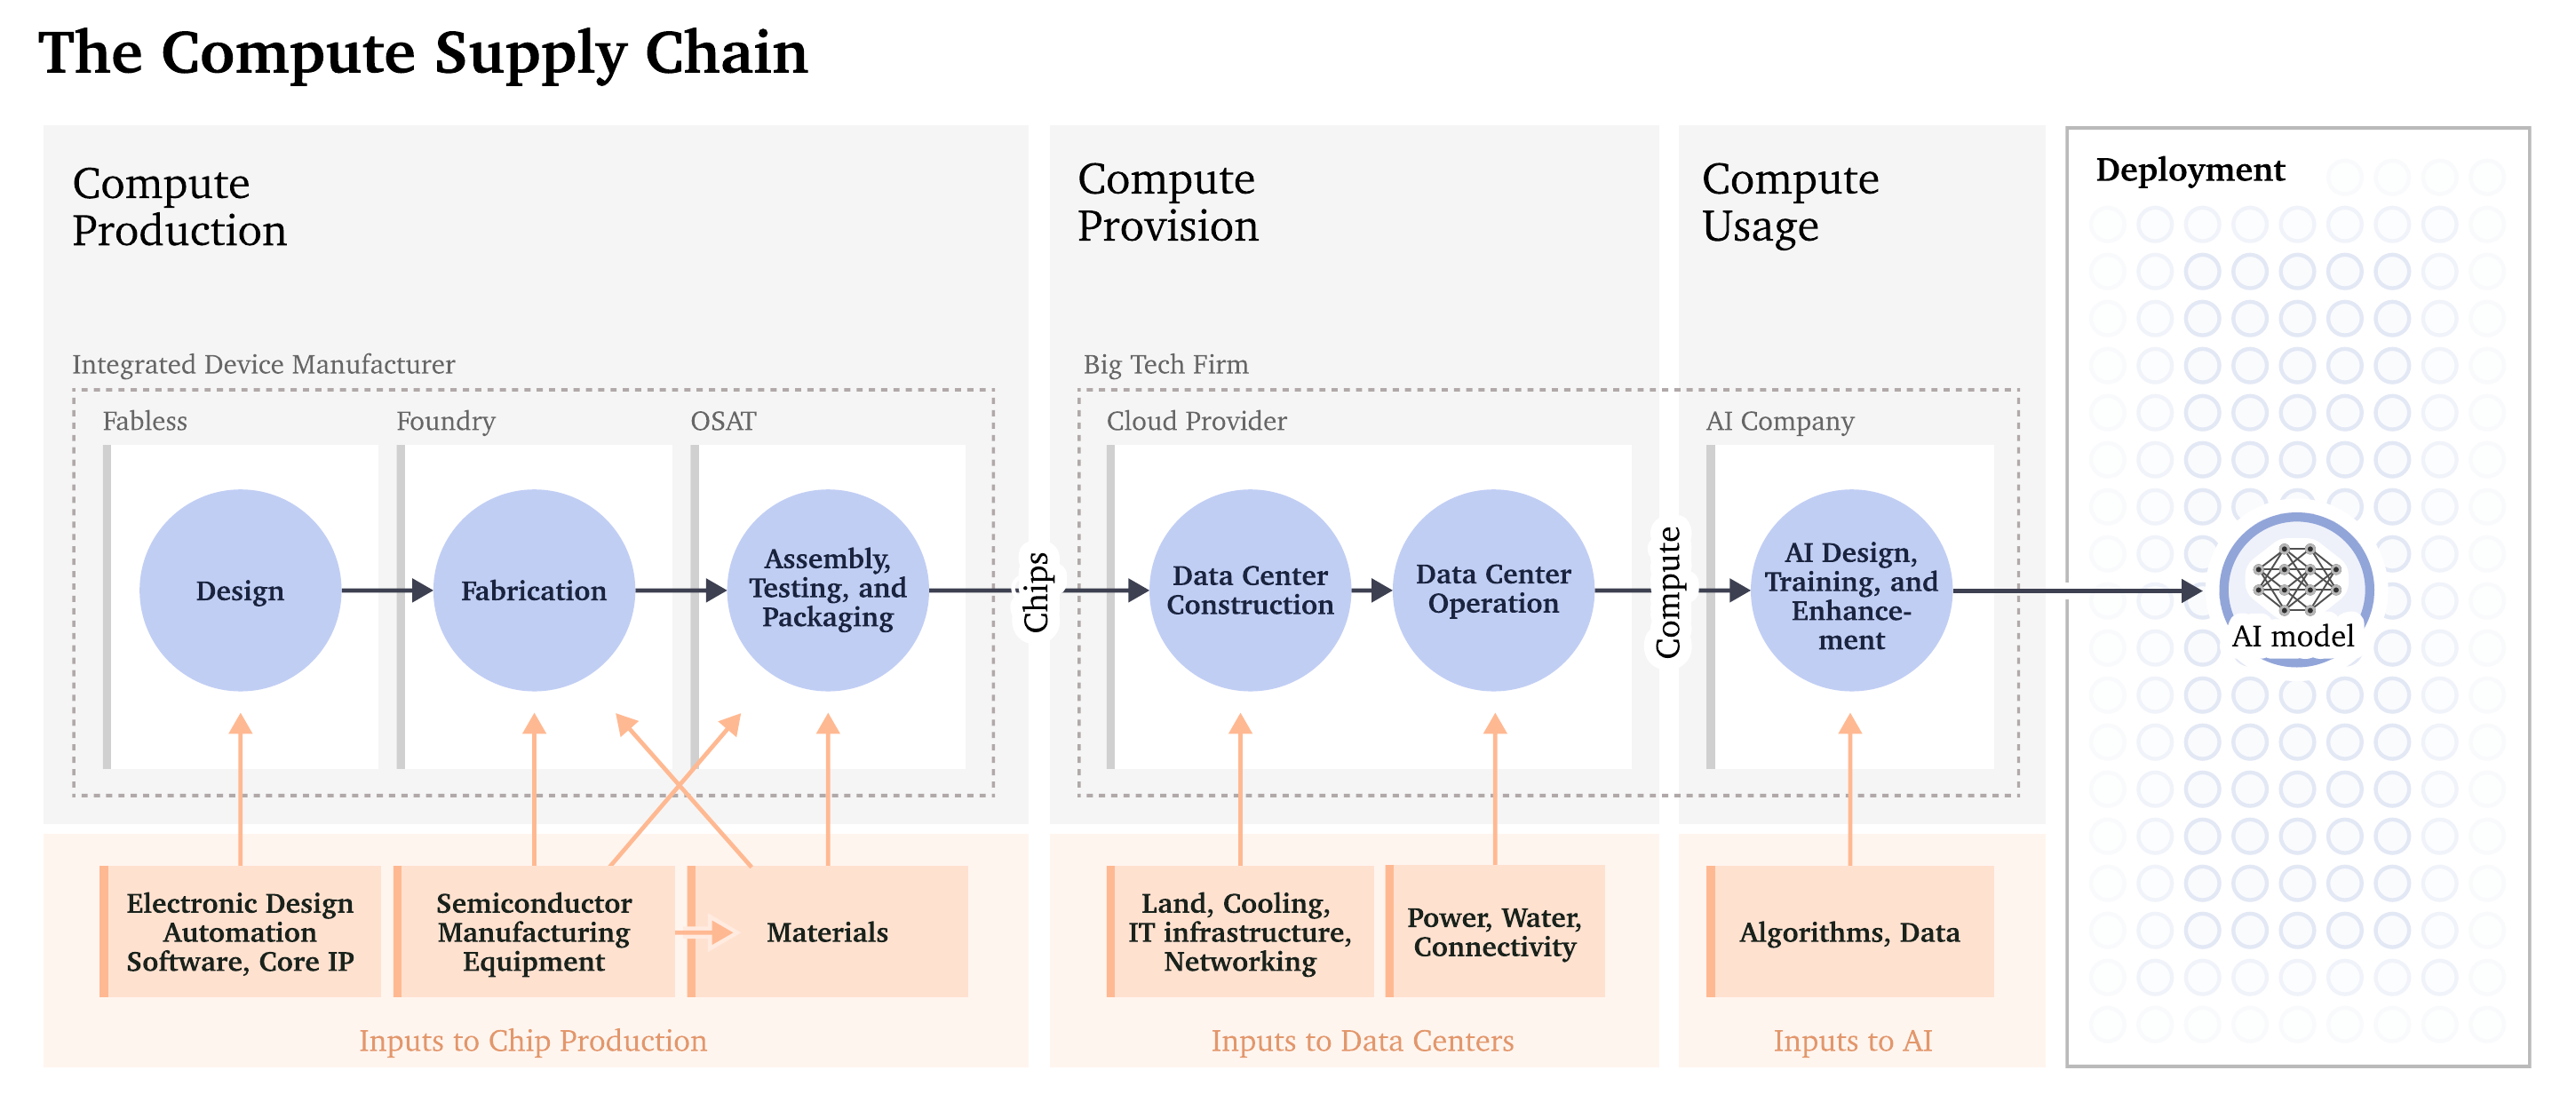
\includegraphics[width=\textwidth]{sastry2024_fig10_compute_supply_chain}
\source{sastry2024}
\end{frame}

\begin{frame}{Compute Is Growing Exponentially}
\begin{columns}[c]
\column{0.5\textwidth}
\centering
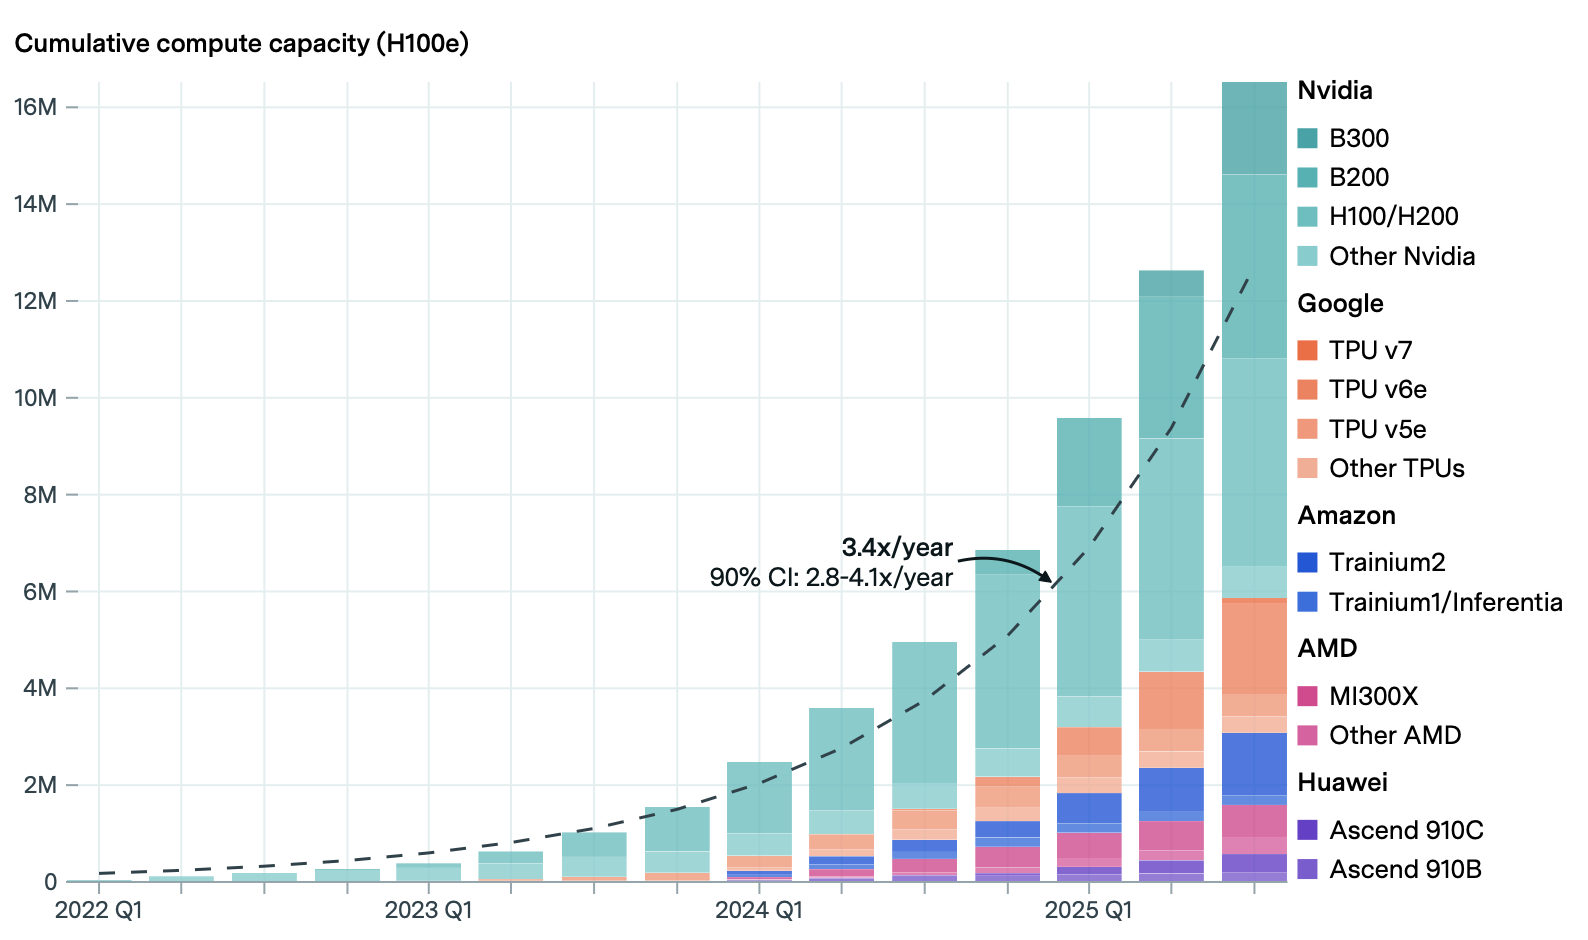
\includegraphics[width=\linewidth]{epoch_chip_stock}

{\small All AI chips in the world: \textbf{3.4$\times$ per year}}
\column{0.5\textwidth}
\centering
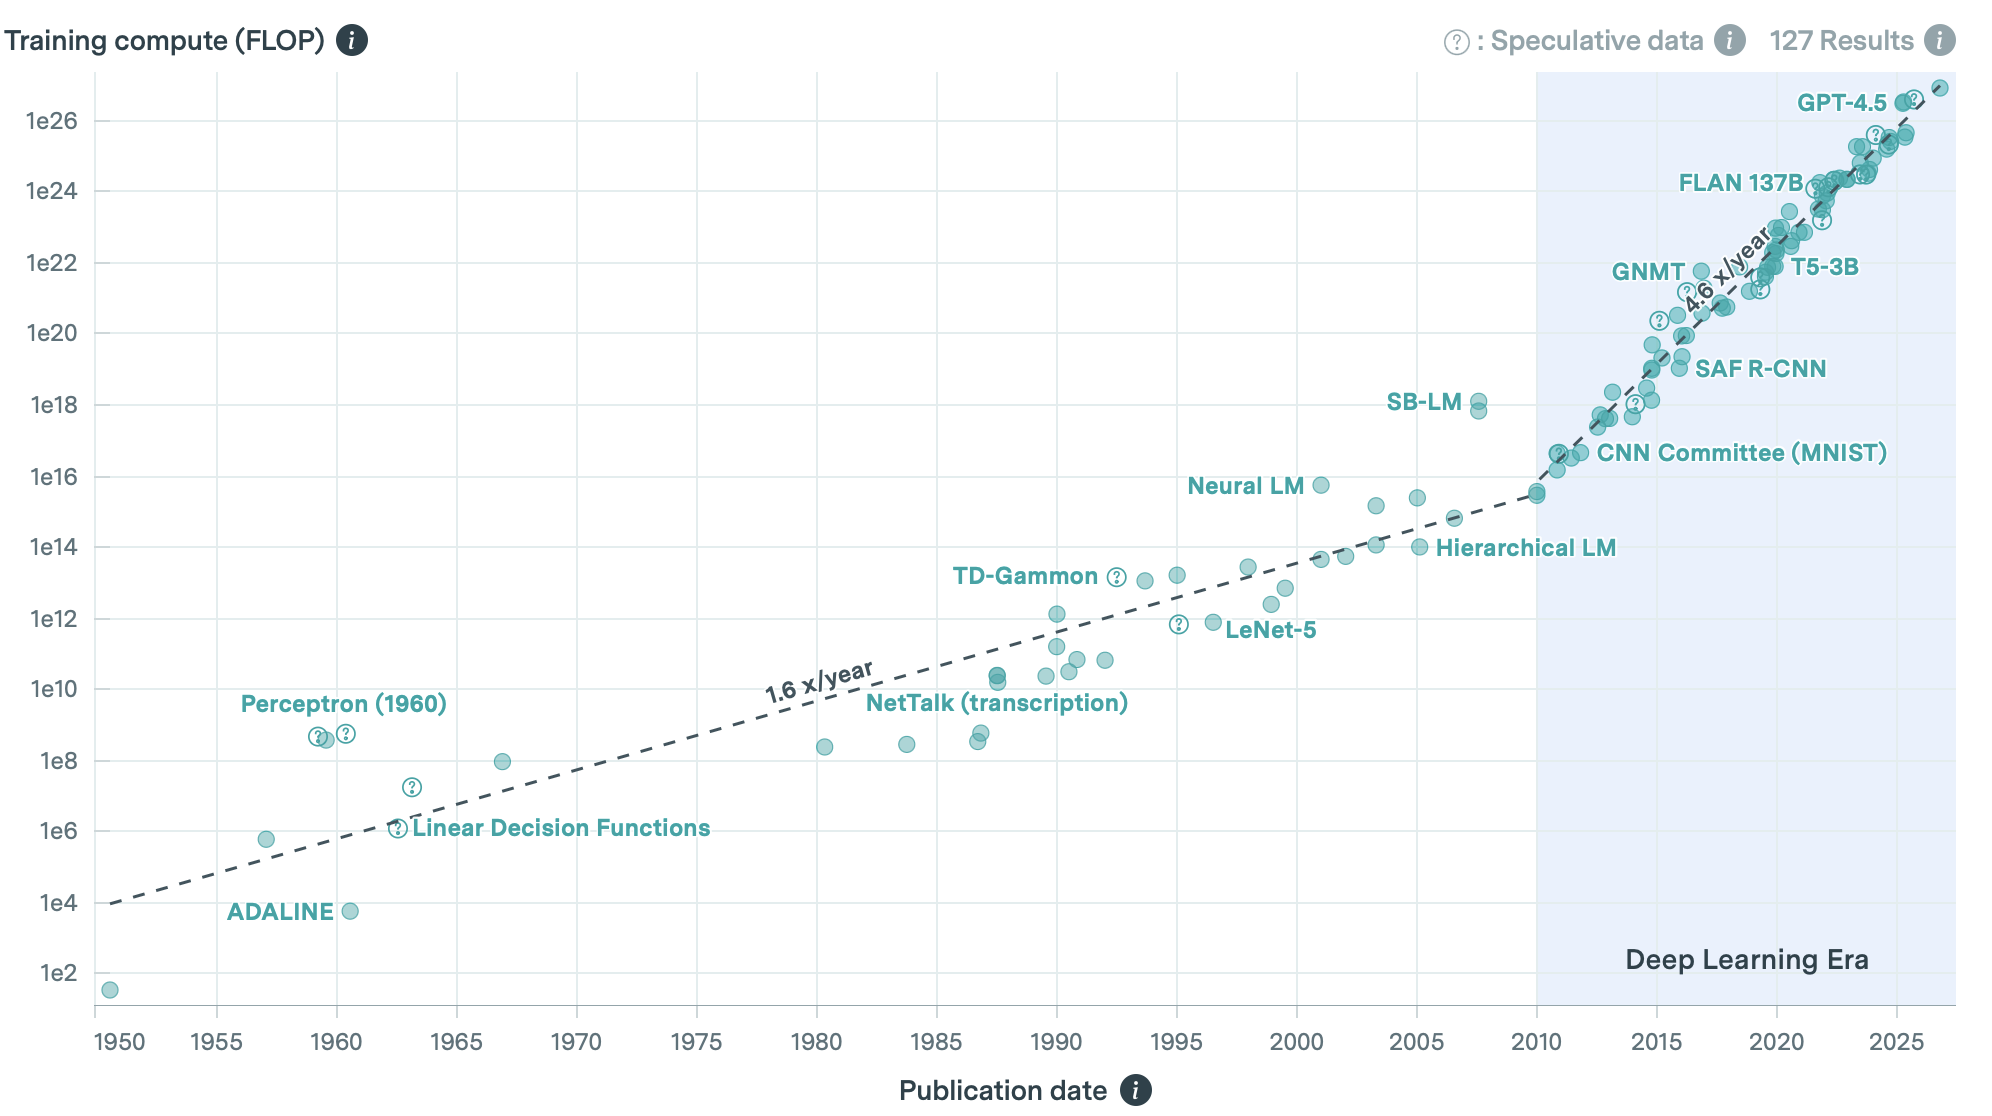
\includegraphics[width=\linewidth]{epoch_training_compute}

{\small Largest training runs: \textbf{4.6$\times$ per year}}
\end{columns}
\source{epochtrends2026,epochmodels2026}
\end{frame}

\begin{frame}{Algorithms Are Improving Exponentially}
\begin{columns}[c]
\column{0.42\textwidth}
\centering
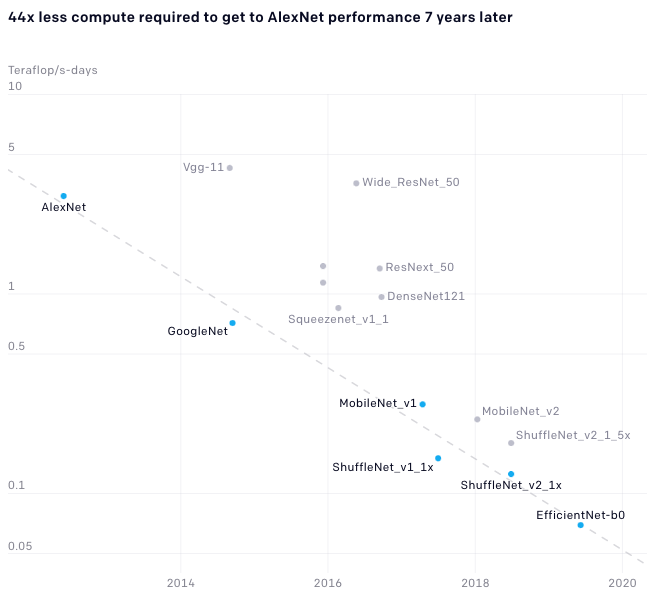
\includegraphics[width=\linewidth]{hernandez_alexnet_efficiency}

{\small Image recognition, 2012--2019:\\ \textbf{44$\times$ less compute}}
\column{0.56\textwidth}
\centering
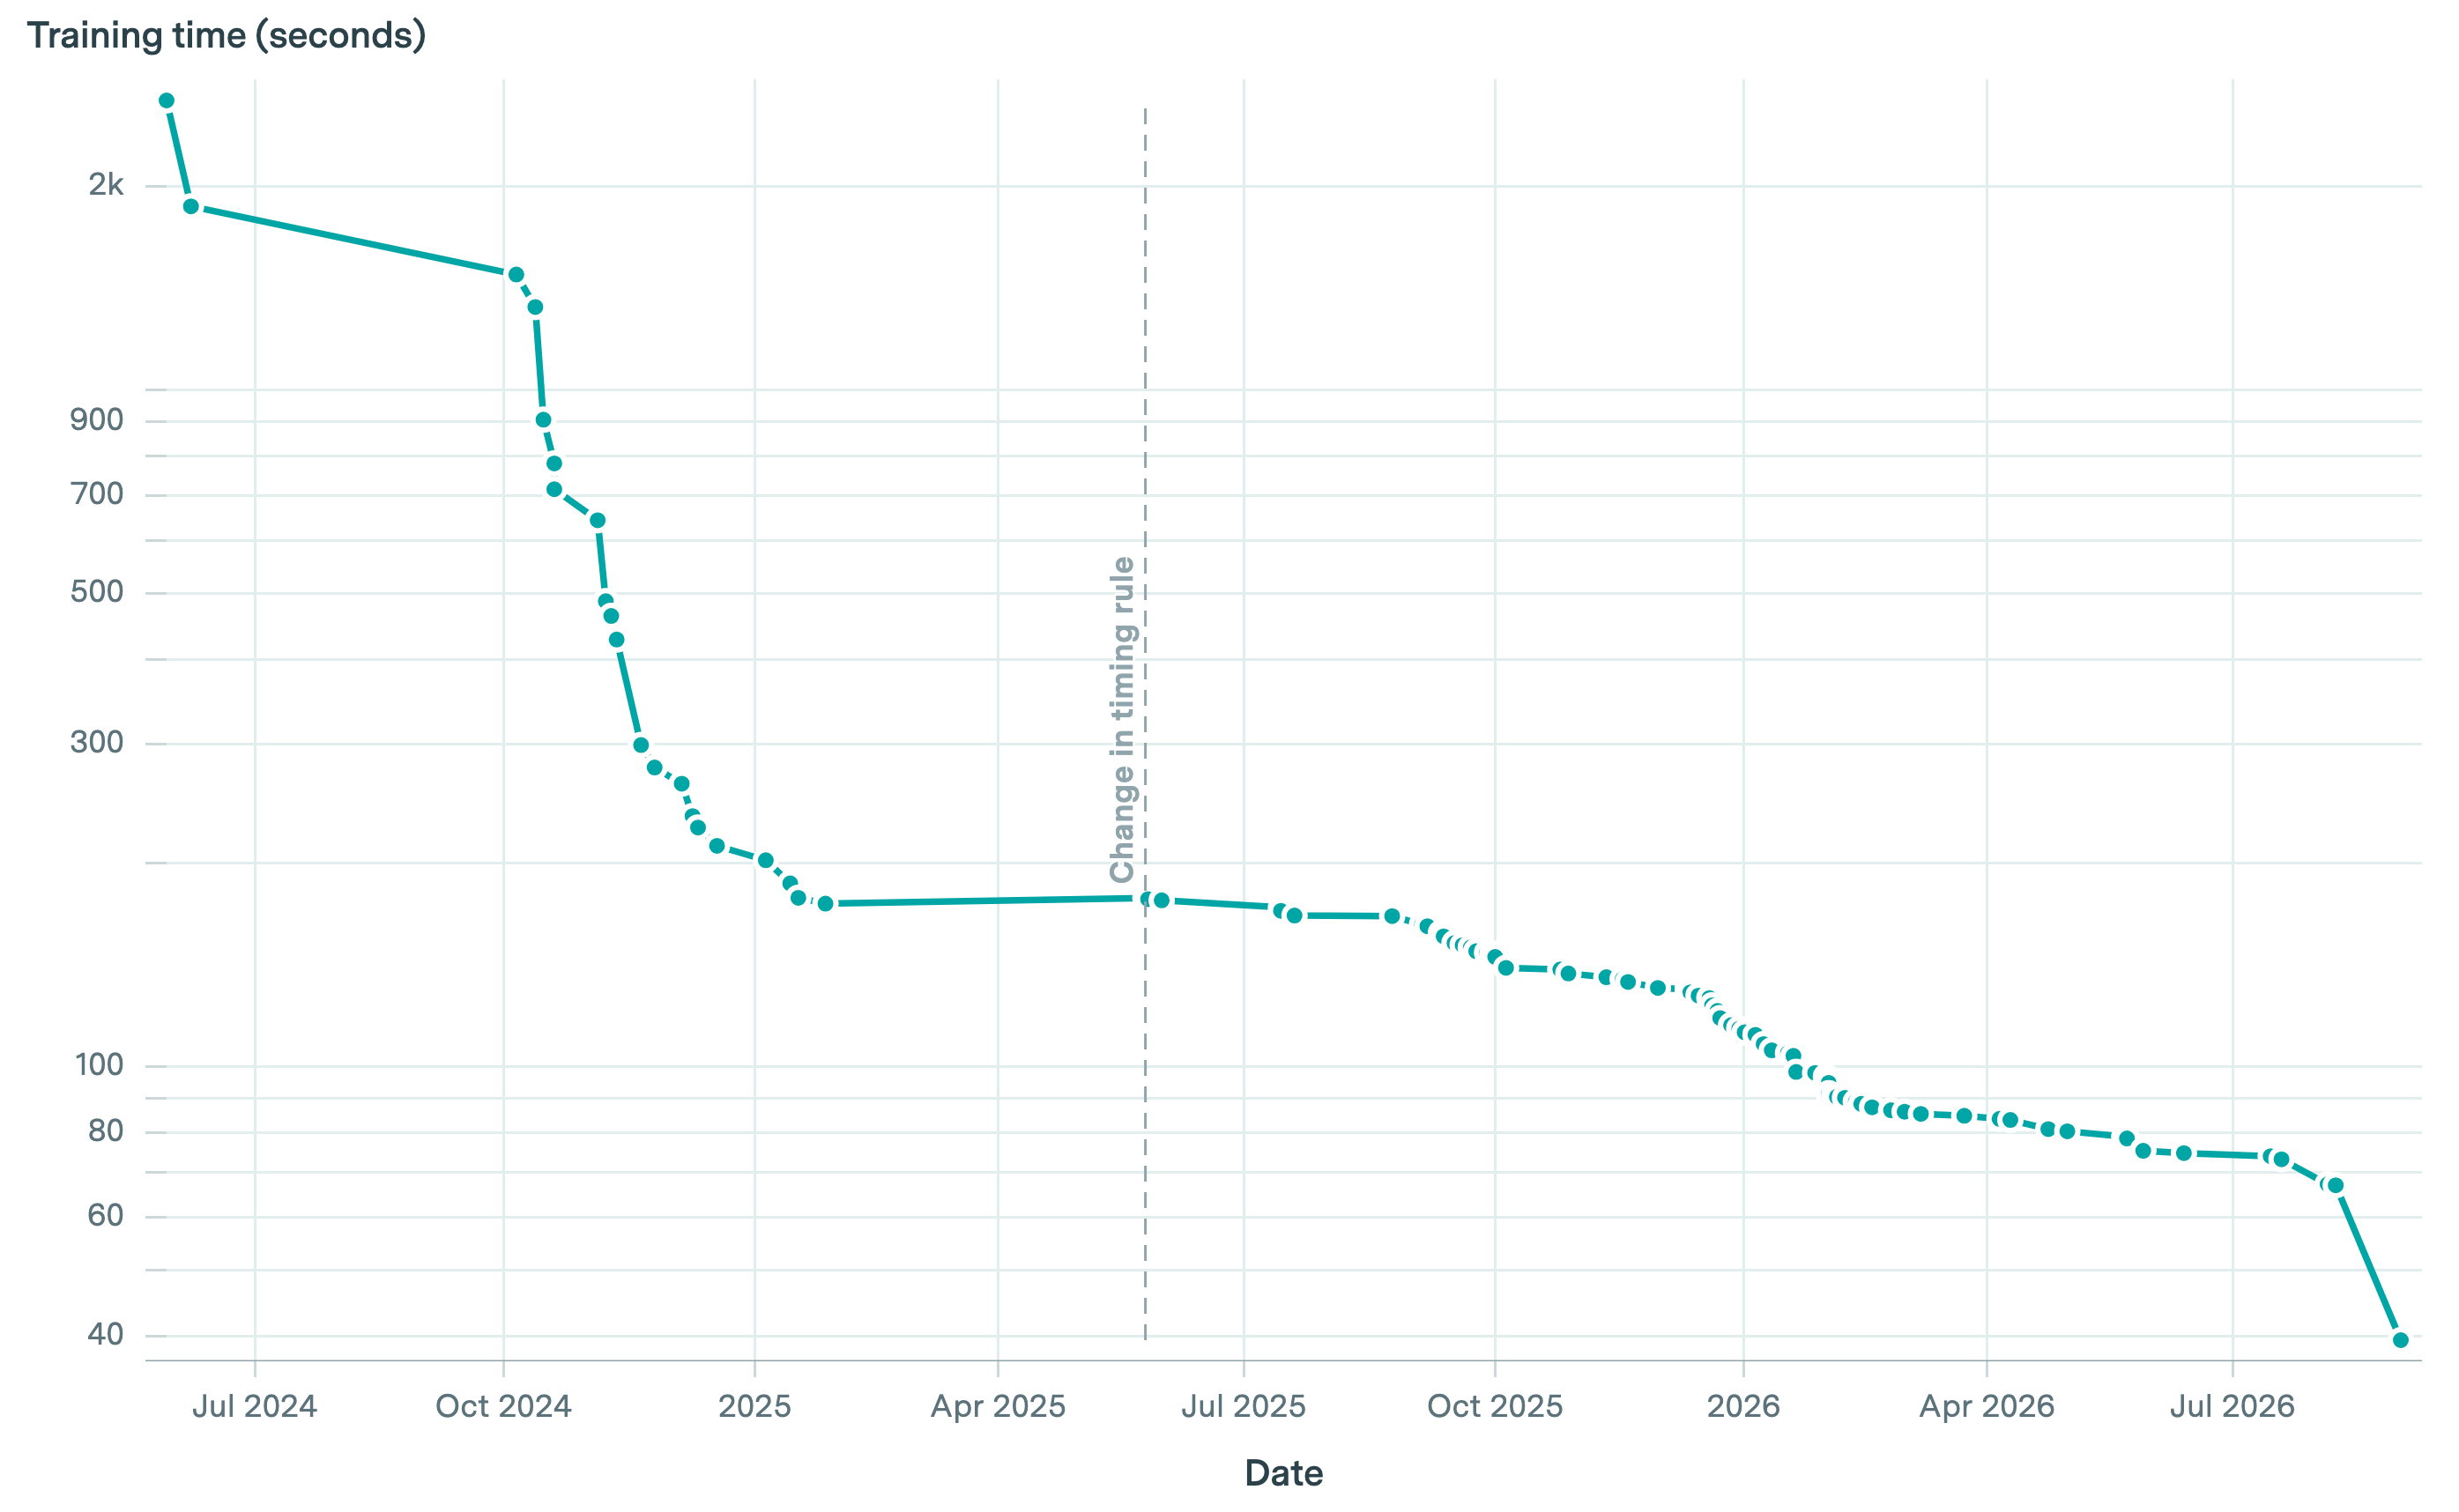
\includegraphics[width=\linewidth]{epoch_nanogpt_speedrun}

{\small Same model, same hardware, same data, 2024--2026:\\ \textbf{45 minutes $\to$ 40 seconds}}
\end{columns}
\source{hernandez2020,ai2026}
\end{frame}

\begin{frame}{Not All Inputs Depend on AI in the Same Way}
\begin{columns}[c]
\column{0.5\textwidth}
\centering
\textbf{Weak recursion}

\vspace{0.6em}
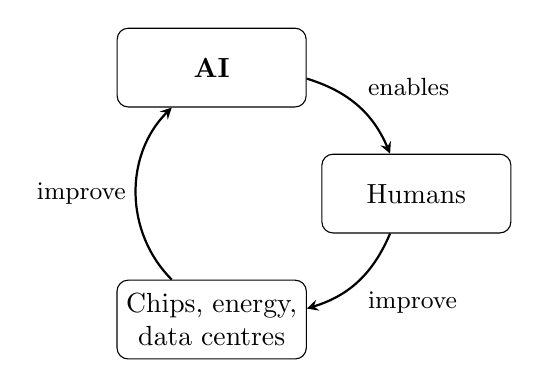
\begin{tikzpicture}[box/.style={draw, rounded corners, align=center, minimum height=1cm, minimum width=2.4cm}, >=stealth]
\node[box] (ai) at (0,3.2) {\textbf{AI}};
\node[box] (h) at (2.6,1.6) {Humans};
\node[box] (hw) at (0,0) {Chips, energy,\\data centres};
\draw[->, thick] (ai) to[bend left=25] node[above right] {\small enables} (h);
\draw[->, thick] (h) to[bend left=25] node[below right] {\small improve} (hw);
\draw[->, thick] (hw) to[bend left=45] node[left] {\small improve} (ai);
\end{tikzpicture}

\vspace{0.8em}
Through the human economy: \textbf{slow}
\column{0.5\textwidth}
\centering
\textbf{Strong recursion}

\vspace{0.6em}
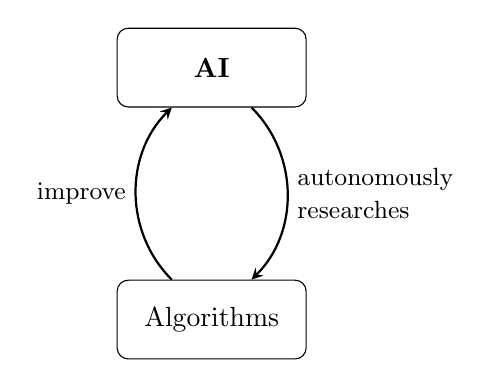
\begin{tikzpicture}[box/.style={draw, rounded corners, align=center, minimum height=1cm, minimum width=2.4cm}, >=stealth]
\node[box] (ai) at (0,3.2) {\textbf{AI}};
\node[box] (alg) at (0,0) {Algorithms};
\draw[->, thick] (ai) to[bend left=45] node[right, align=left] {\small autonomously\\\small researches} (alg);
\draw[->, thick] (alg) to[bend left=45] node[left] {\small improve} (ai);
\end{tikzpicture}

\vspace{0.8em}
Inside the data centre: \textbf{fast}
\end{columns}
\source{ball2026}
\end{frame}

\begin{frame}{Can an AI Build a Smarter AI?}
\begin{center}
\begin{tikzpicture}[scale=0.88, >=stealth]
\useasboundingbox (-1.5,-0.3) rectangle (11.5,7.7);
\draw[->] (0.4,0.4) -- (7.6,0.4) node[below left] {\small Intelligence of the AI doing the research};
\draw[->] (0.4,0.4) -- (0.4,7.3) node[above right, xshift=-0.3cm] {\small Smartest AI it can build};
\draw[gray, dashed] (0.4,0.4) -- (7,7) node[right, text=gray] {\small as smart as itself};
\only<1-5>{\draw[very thick, domain=1.3:4.3, samples=50] plot (\x, {\x + 0.5*(\x-2)*(4-\x)});}
\only<2>{
  \draw[thick, red!70!black, ->] (1.60,1.60) -- (1.60,1.12) -- (1.12,1.12);
  \node[red!70!black, align=left, anchor=west] at (2.6,1.2) {\small A weaker AI builds\\\small a weaker successor};
}
\only<3-5>{
  \draw[thick, green!50!black] (2.40,2.40) -- (2.40,2.72) -- (2.72,2.72);
  \node[green!50!black, align=left, anchor=west] at (4.6,2.6) {\small A stronger AI builds\\\small a stronger successor};
}
\only<4-5>{\draw[thick, green!50!black] (2.72,2.72) -- (2.72,3.18) -- (3.18,3.18);}
\only<5>{
  \draw[thick, green!50!black, ->] (3.18,3.18) -- (3.18,3.66) -- (3.66,3.66) -- (3.66,3.94) -- (3.94,3.94) -- (3.94,4.00) -- (4.00,4.00);
  \node[anchor=west] at (4.2,3.9) {\small the loop runs out of steam};
}
\only<6>{
  \draw[gray, domain=1.3:4.3, samples=50] plot (\x, {\x + 0.5*(\x-2)*(4-\x)});
  \draw[very thick, domain=1.3:6.9, samples=50] plot (\x, {\x + 0.222*(\x-2)*(6.5-\x)});
  \draw[thick, green!50!black, ->] (2.40,2.40) -- (2.40,2.76) -- (2.76,2.76) -- (2.76,3.40) -- (3.40,3.40) -- (3.40,4.36) -- (4.36,4.36) -- (4.36,5.48) -- (5.48,5.48) -- (5.48,6.27) -- (6.27,6.27) -- (6.27,6.49) -- (6.49,6.49) -- (6.49,6.50) -- (6.50,6.50);
  \node[anchor=north west] at (6.5,6.4) {\small limit of current hardware};
}
\end{tikzpicture}
\end{center}
\end{frame}

\begin{frame}{How Could This Play Out?}
\centering
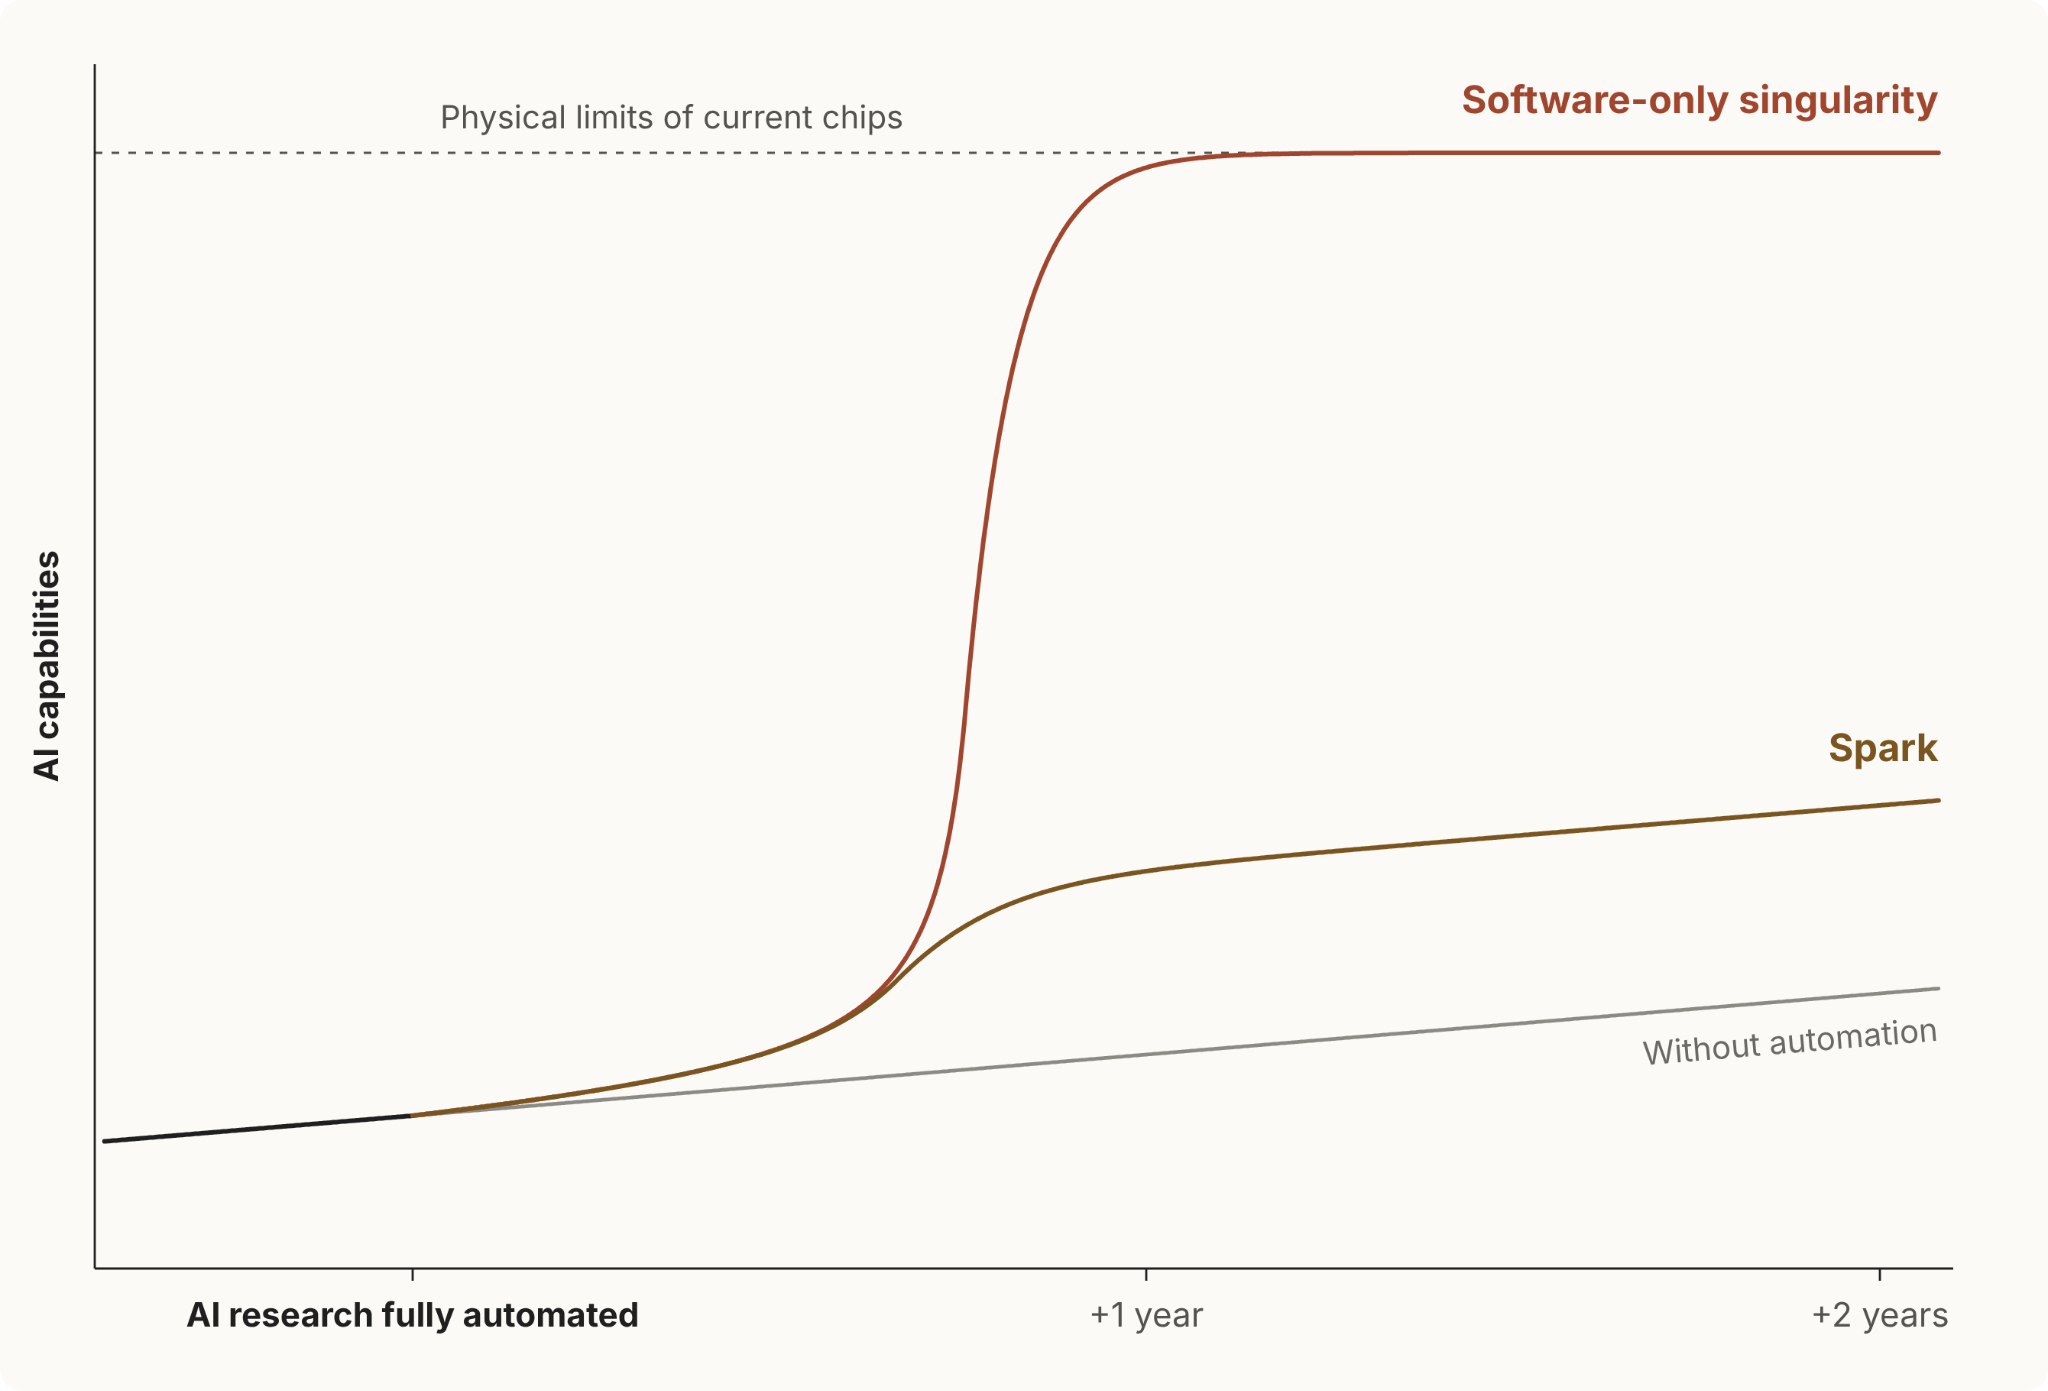
\includegraphics[height=0.78\textheight]{takeoff_scenarios}

\source{patel2026}
\end{frame}

\begin{frame}{Intuition Pump: What Just Happened in Maths}
\begin{columns}[t]
\column{0.2\textwidth}
\centering
{\LARGE\textbf{2023}}

\vspace{1.2em}
{\Large
\begin{tabular}{@{}r@{}}
4817\\
+\,2956\\
\hline
?
\end{tabular}}

\vspace{1em}
{\scriptsize Four-digit addition}
\column{0.24\textwidth}
\centering
\onslide<2->{
{\LARGE\textbf{2024}}

\vspace{1.2em}
\fbox{\parbox{0.9\linewidth}{\raggedright\tiny Janet's ducks lay 16 eggs per day. She eats three for breakfast every morning and bakes muffins for her friends every day with four. She sells the remainder at the farmers' market daily for \$2 per fresh duck egg. How much in dollars does she make every day at the farmers' market?}}

\vspace{1em}
{\scriptsize Grade school word problems}
}
\column{0.26\textwidth}
\centering
\onslide<3->{
{\LARGE\textbf{2025}}

\vspace{1.2em}
\fbox{\parbox{0.9\linewidth}{\raggedright\tiny A line in the plane is called \emph{sunny} if it is not parallel to any of the $x$-axis, the $y$-axis, and the line $x+y=0$. Let $n\ge 3$ be a given integer. Determine all nonnegative integers $k$ such that there exist $n$ distinct lines in the plane satisfying both of the following: for all positive integers $a$ and $b$ with $a+b\le n+1$, the point $(a,b)$ is on at least one of the lines; and exactly $k$ of the $n$ lines are sunny.}}

\vspace{0.4em}

\begin{tikzpicture}
\fill[red!70!black] (-0.22,0.25) -- (-0.4,0.9) -- (-0.1,0.9) -- (0,0.45) -- (0.1,0.9) -- (0.4,0.9) -- (0.22,0.25) -- cycle;
\fill[yellow!70!orange] (0,0) circle (0.36);
\draw[orange!80!black, thick] (0,0) circle (0.36);
\node[orange!50!black] at (0,0) {\small\textbf{1}};
\end{tikzpicture}

{\scriptsize Gold at the Maths Olympiad}
}
\column{0.26\textwidth}
\centering
\onslide<4->{
{\LARGE\textbf{2026}}

\vspace{0.4em}
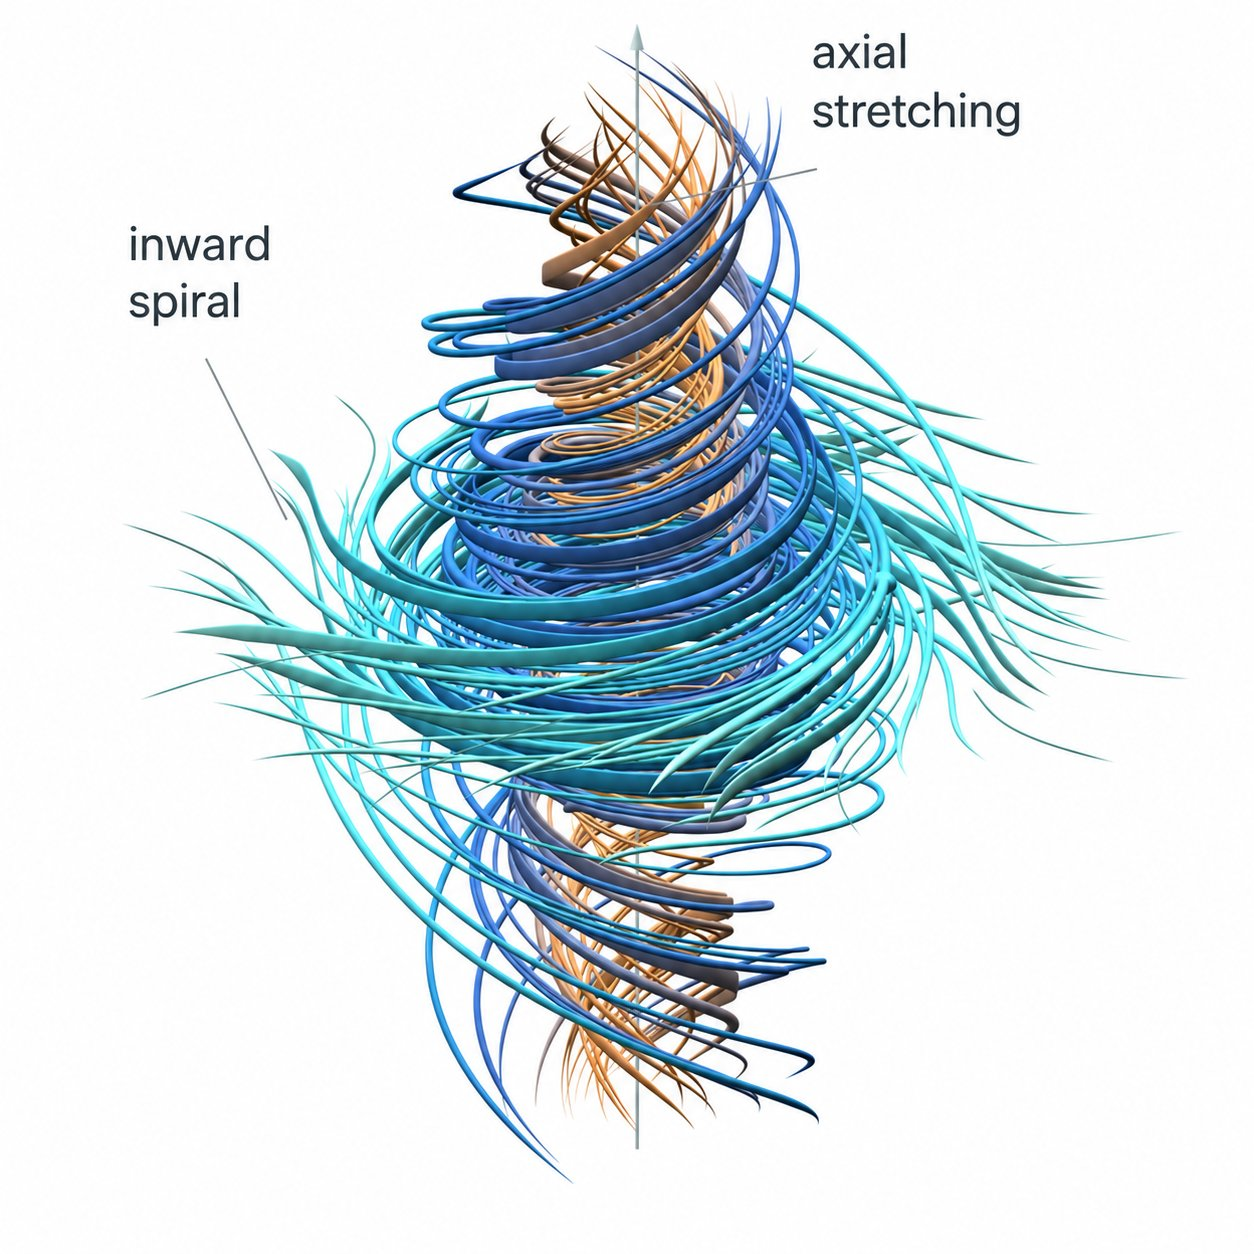
\includegraphics[width=0.95\linewidth]{openai_navier_stokes}

{\scriptsize Navier--Stokes,\\a Millennium Prize Problem}
}
\end{columns}
\source{openai2026navierstokes}
\end{frame}

\begin{frame}{Years of Maths Progress in One Release}
\centering
\includegraphics<1>[width=\textwidth]{maths_decade_stage1}%
\includegraphics<2>[width=\textwidth]{maths_decade_stage2}

{\raggedright\scriptsize \onslide<2>{Orange: claimed by OpenAI, largely not yet independently verified.}\par}
\source{wikipedia2026solved,wikipedia2026bulk}
\end{frame}

\begin{frame}{Machine Learning Is a Young Field}
\begin{center}
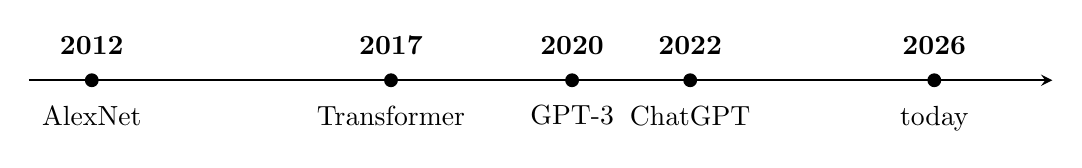
\begin{tikzpicture}[>=stealth]
\draw[->, thick] (0,0) -- (13,0);
\foreach \x/\y/\n in {0.8/2012/AlexNet, 4.6/2017/Transformer, 6.9/2020/GPT-3, 8.4/2022/ChatGPT, 11.5/2026/today} {
  \fill (\x,0) circle (2.5pt);
  \node[above=0.2cm] at (\x,0) {\textbf{\y}};
  \node[below=0.2cm] at (\x,0) {\n};
}
\end{tikzpicture}
\end{center}
\vspace{1.5em}
\centering
What would decades of progress in \emph{this} field look like?
\end{frame}

\begin{frame}{But Maths Was Not Recursive}
\begin{columns}[c]
\column{0.48\textwidth}
\centering
\begin{tikzpicture}[every node/.style={draw, rounded corners, align=center, minimum height=1cm, minimum width=2.2cm}, >=stealth]
\node (a) {AI};
\node (b) [right=1.5cm of a] {Maths\\results};
\draw[->, thick] (a) -- (b);
\end{tikzpicture}

\vspace{1em}
Proving theorems does not make\\the AI better at proving theorems
\column{0.48\textwidth}
\centering
\begin{tikzpicture}[every node/.style={draw, rounded corners, align=center, minimum height=1cm, minimum width=2.2cm}, >=stealth]
\node (a) {AI};
\node (b) [right=1.5cm of a] {ML\\results};
\draw[->, thick, bend left=35] (a) to (b);
\draw[->, thick, bend left=35] (b) to (a);
\end{tikzpicture}

\vspace{1em}
Doing ML research makes\\the AI better at ML research
\end{columns}
\end{frame}

\begin{frame}{Examples of Recursive Growth?}
\centering
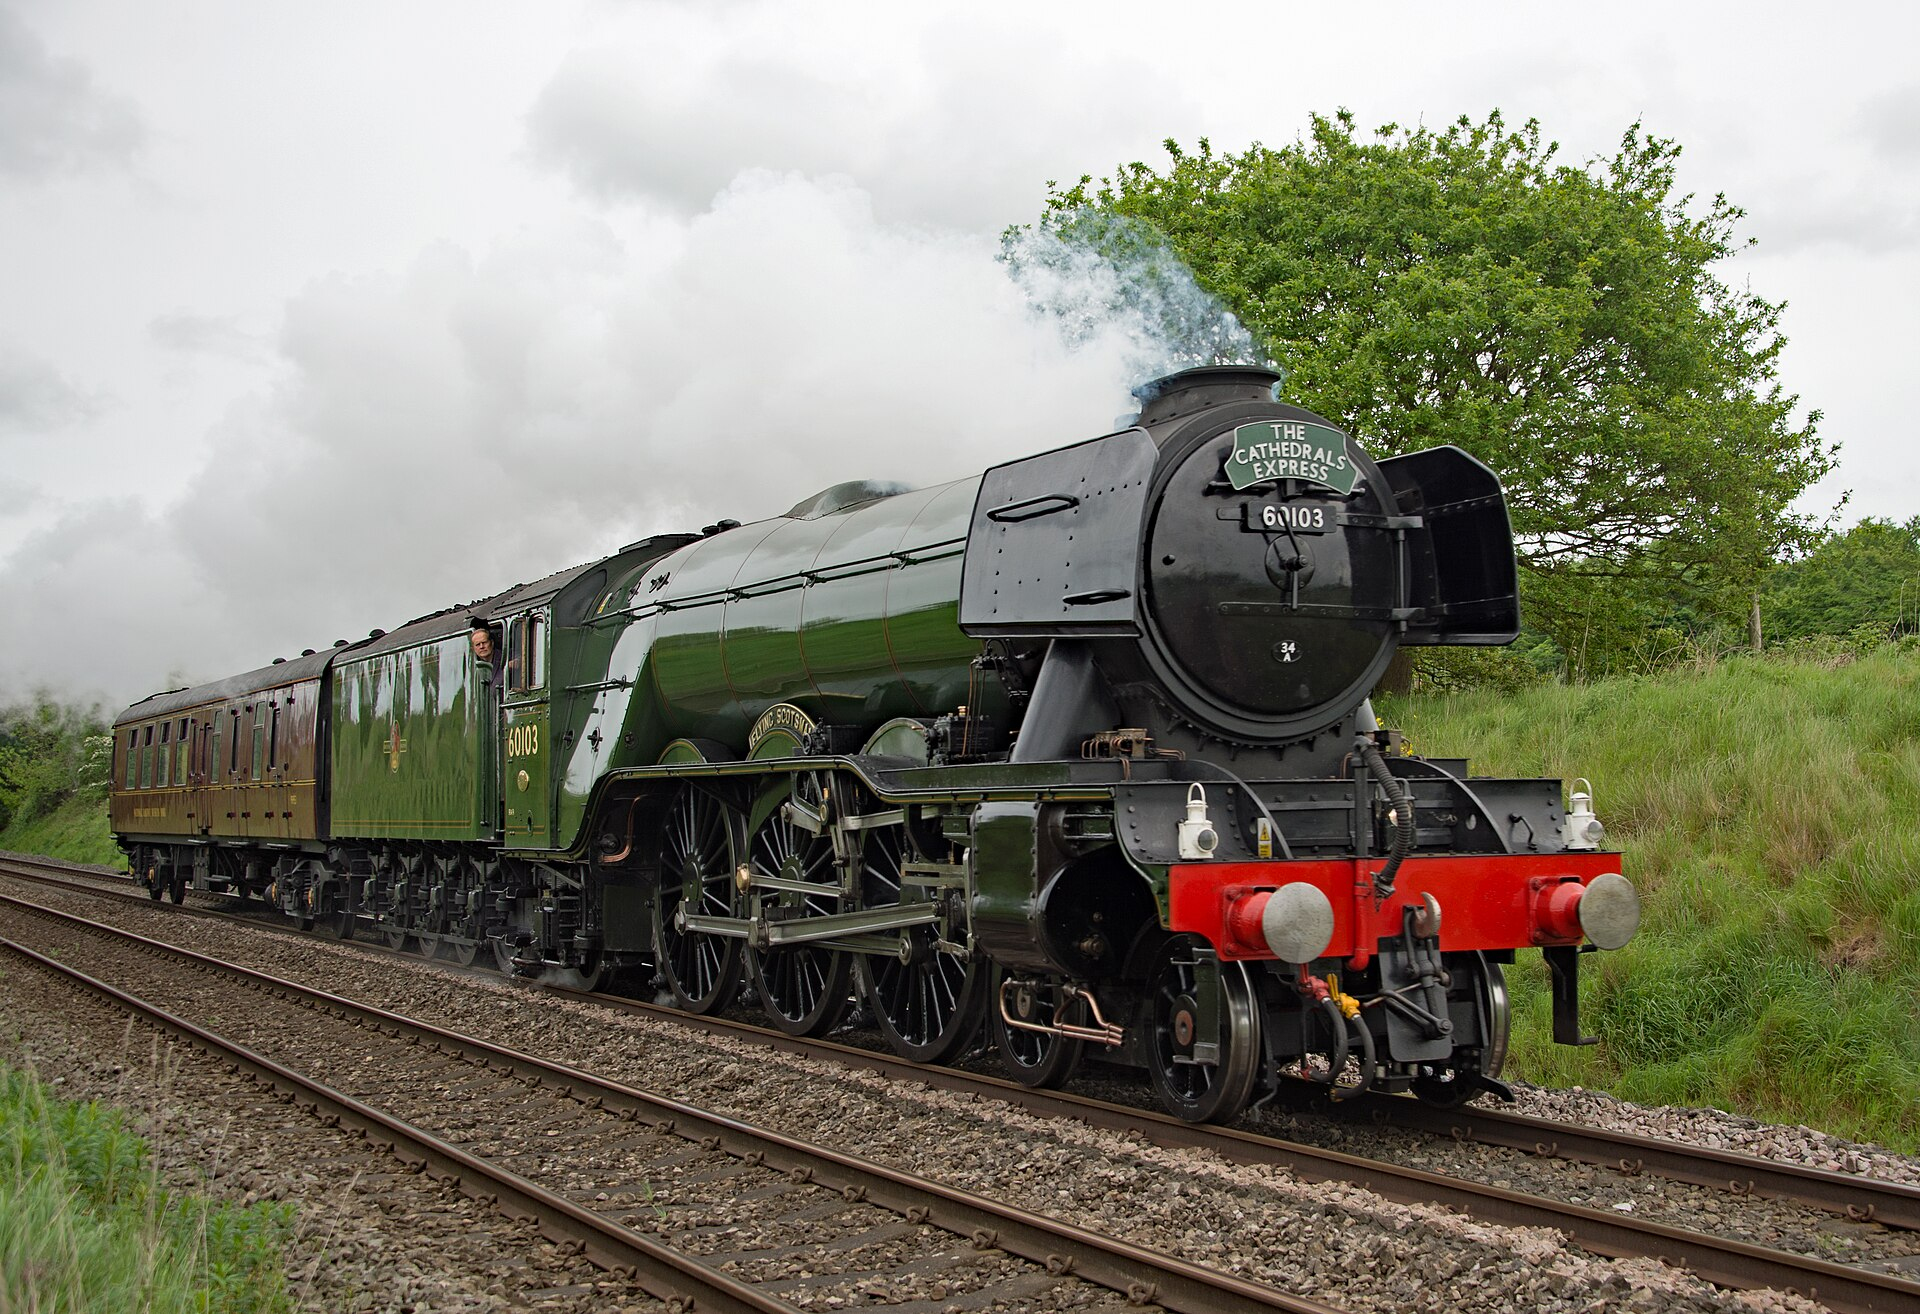
\includegraphics[height=0.52\textheight]{train}

{\tiny\color{gray}Photo: ARG\_Flickr, CC BY 2.0}

\vspace{0.6em}
{\large Would AI be the next Industrial Revolution?}

\vspace{0.6em}
\onslide<2->{{\large No. The Industrial Revolution and other technologies were only \textbf{weak recursion}.}}
\end{frame}

\begin{frame}{The Closest Precedent: Humans}
\begin{columns}[c]
\column{0.5\textwidth}
\centering
\begin{tikzpicture}[>=stealth, slow/.style={blue!70!black}, fast/.style={red!75!black}]
\node (top) at (0,3) {\Huge\faDna};
\node[above=0.1cm of top] {\textbf{Evolution}};
\node (bot) at (0,0) {\Huge\faUser};
\draw[->, very thick, slow] (top) -- node[left, align=right] {natural selection\\\textbf{slow}} (bot);
\draw[->, very thick, fast] (bot.east) to[out=30, in=-30, looseness=6] node[right, align=left] {cultural evolution\\\textbf{fast}} (bot.south east);
\end{tikzpicture}
\column{0.5\textwidth}
\centering
\begin{tikzpicture}[>=stealth, slow/.style={blue!70!black}, fast/.style={red!75!black}]
\node (top) at (0,3) {\Huge\faUser};
\node[above=0.1cm of top] {\textbf{Humans}};
\node (bot) at (0,0) {\Huge\faRobot};
\draw[->, very thick, slow] (top) -- node[left, align=right] {training models\\\textbf{slow}} (bot);
\draw[->, very thick, fast] (bot.east) to[out=30, in=-30, looseness=6] node[right, align=left] {RSI\\\textbf{fast}} (bot.south east);
\end{tikzpicture}
\end{columns}
\end{frame}
